\section{Light deflection}
\label{sec:light_deflection}

According to Einstein's theory of relativity, objects with gravitational pull have the ability to alter the fabric of space-time, resulting in the bending of light rays \citep{narayan_lectures_1997}
. Gravitational lensing occurs when a substantial mass distribution can effectively curve and amplify the light emitted from a source positioned behind it.

The calculation of light deflection involves the examination of geodesic curves originating from the field equations of general relativity. Light deflection can also be understood through Fermat's principle\footnote{Light travels between two points along the path that requires the least time.}, similar to how it is described in geometrical optics. The main approach is to consider light deflection within the framework of general relativity as a refraction problem, for which a refractive index \emph{n} can be introduced.

To investigate the bending of light and to determine the refractive index, an initial approximation is made by assuming that the lens is ``weak'' and significantly smaller than the source-lens-observer optical system, an assumption true for nearly all astrophysical scenarios. This ``weak field'' approximation refers to a lens with a relatively small Newtonian gravitational potential, which means $\f \ll c^2$, where $c$ is the speed of light.
Additionally, it is plausible to assume that light deflection occurs within a region small enough that the expansion of the universe can be disregarded. Leveraging the principle of equivalence, one can select a locally inertial frame in which space-time is flat and described by Minkowski's metric. In this context, the line element of the local metric tensor can be written as a small perturbation of the metric, such as
\be
\label{eq:2.1}
\dd{s}^2 = g_{\m\n} \dd{x}^\m \dd{x}^\n = \bp{1 + \frac{2\f}{c^2}} c^2 \dd{t}^2 - \bp{1 - \frac{2\f}{c^2}} \dd{\vec{x}}^2 \,.
\ee

Since light travels on null geodesics, for which $\dd{s}^2 = 0$, the light speed in the gravitational perturbation is thus
\be
\label{eq:2.2}
c^\prime = \frac{\dd{\vec{x}}}{\dd{t}} \approx c \bp{1 + \frac{2 \f}{c^2}} \,,
\ee
and given that $\f \leq 0$, $c^\prime$ is smaller than in the absence of a gravitational potential.

This leads to the definition of the \emph{effective refraction index} as
\be
\label{eq:2.3}
n = \frac{c}{c^\prime} \approx 1 - \frac{2\f}{c^2} \geq 1 \,.
\ee
    
Applying Fermat's principle, the total deflection angle of a photon is the integral over the gradient of the potential perpendicular to the light path along the proper light path. Thanks to the \emph{Born approximation}\footnote{Simplification valid when the gravitational potential is small: deflection of light is treated like a linear process, neglecting higher-order corrections.}, it can be shown \citep{schneider_gravitational_1992} that the deflection angle can be obtained integrating over the unperturbed light path:
\be
\label{eq:2.4}
\hat{\va{\a}} (\va{\x}) = \frac{2}{c^2} \int_{-\infty}^{+\infty} \va{\nabla}_\perp \f (\va{\x}, z) \dd{z} \,,
\ee   
where $\x$ is the impact parameter of the photon traveling along the $\vec{e}_z$ direction that passes through the lens at $z=0$ (\cref{fig:bornapprox}).

\begin{figure}
    \centering
    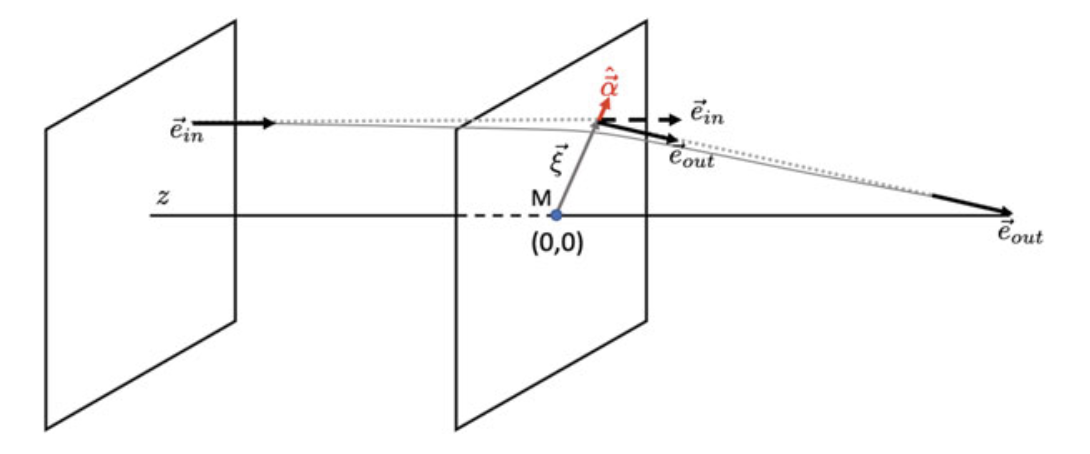
\includegraphics[width=\linewidth, keepaspectratio]{img//chapter2/bornapprox.png}
    \caption[Born approximation schematics]{Schematics for the Born approximation.\\\small{Credits: \cite{meneghetti_introduction_2021}.}}
    \label{fig:bornapprox}
\end{figure}

If the lens can be approximated by a point mass, the potential is $\f = -\frac{G M}{\sqrt{\x^2 + z^2}}$, where $G$ is the gravitational constant, and thus \cref{eq:2.4} simplifies to the following:
\be
\label{eq:2.5}
\hat{\va{\a}} (\va{\x}) = \frac{4 G M}{c^2 \x} \vec{e}_\x = \frac{4 G M}{c^2 \x^2} \va{\x} \;.
\ee

Under the assumption of weak field, the superposition principle can be applied to extend the previous definition to calculate the deflection angle of an ensemble of point-like lenses. Having a sparse distribution of $N$ point masses on a plane, the deflection angle of a light ray crossing the plane at $\va{\x}$ will be
\be
\label{eq:2.6}
\hat{\va{\a}} (\va{\x}) = \sum_i^N \hat{\va{\a}}_i (\va{\x} - \va{\x}_i) = \frac{4 G}{c^2} \sum_i^N M_i \frac{\va{\x} - \va{\x}_i}{{|\va{\x} - \va{\x}_i|}^2} \,,
\ee
where $\va{\x}_i$ and $M_i$ are the positions and masses of each lens.

When discussing more realistic situations of lensing, such as those involving three-dimensional distributions of matter, it is important to note that the physical extent of the lens is typically much smaller than the distances between the observer, the lens, and the source. Consequently, the bending of light occurs primarily over a brief segment of its path. This observation allows for the application of the \emph{thin screen approximation}, where the lens is represented as a planar distribution of matter, termed the lens plane. In this simplified model, the distribution of matter responsible for lensing is completely characterized by its surface density
\be
\label{eq:2.7}
\S (\va{\x}) = \int \r (\va{\x}, z) \dd{z} \,,
\ee
where $\va{\x}$ is a two-dimensional vector on the lens plane and $\r$ is the three-dimensional density.

In this context, the total deflection angle can be obtained by summing the contributions of all the mass elements $\S (\va{\x}) \dd^2{\x}$:
\be
\label{eq:2.8}
\hat{\va{\a}} (\va{\x}) = \frac{4 G}{c^2} \int \frac{(\va{\x} - \va{\x}^\prime) \S (\va{\x}^\prime)}{{|\va{\x} - \va{\x}^\prime|}^2} \dd^2{\x^\prime} \,.
\ee